\begin{appendices}
\label{ch:appendices}

\chapter{Objectives Principles Strategies - Effectiveness}

The items marked with \XSolidBrush  are the ones not included in the surveys to the teams.

\newcommand*\addition{\item[\FiveStar]}
\newcommand*\indicatorAddition{\item[\FiveStarOutline]}
\newcommand*\strategyAddition{\item[\TwelweStar]}
\newcommand*\removed{\item[\XSolidBrush]}

%\begin{itemize}
%	\item Refactoring
%		\begin{itemize}
%			\item Support for Refactoring 
%				\begin{itemize}
%					\item Is refactoring an expected activity?
%					\item Is it feasible to implement code refactoring?
%					\item Is it feasible to implement architecture refactoring?
%				\end{itemize}
%			\item Buy-in for Refactoring
%				\begin{itemize}
%					\item Are the teams receptive to implementing refactoring?
%					\addition Are the teams permitted to refactor anywhere in the code base?
%					\item Is the management receptive to supporting refactoring efforts?
%				\end{itemize}
%			\item Minimizing Technical Debt
%				\begin{itemize}
%					\item Is it expected that a well-defined process be adopted to minimize technical debt?
%					\item Is it expected that a well-defined process be adopted to manage technical debt?
%					\item Is minimizing technical debt a high priority activity?
%				\end{itemize}
%		\end{itemize}	
%%---------------------------------------------------------------------------			
%	\item Distribution of expertise
%		\begin{itemize}
%			\item Appropriate team composition
%				\begin{itemize}
%					\item Is a scheme for appropriate team composition defined?
%					\item Are the requisite skillsets for particular projects identified upfront?
%					\item Is it expected that the right people be chosen to accomplish the tasks?
%				\end{itemize}
%		\end{itemize}
%%---------------------------------------------------------------------------		
%	\item Configuration Management
%		\begin{itemize}
%			\item Tool Support for Configuration Management
%				\begin{itemize}
%					\item Do tools for version control and management exist?
%				\end{itemize}
%			\item Support for Configuration Management
%				\begin{itemize}
%					\item Is it expected that the code be kept up to date?
%					\item Is it expected that the tests be kept up to date?
%					\item Is it expected that the builds be kept up to date?
%					\item Is it expected that the release infrastructure be kept up to date?
%					\item Is it expected that the documentation be kept up to date?
%				\end{itemize}
%		\end{itemize}
%%---------------------------------------------------------------------------
%	\item Adherence to standards
%		\begin{itemize}
%			\item Identifying features
%				\begin{itemize}
%					\item Is it expected that well-defined techniques be used to identify the features?
%					\end{itemize}
%			\item Estimation
%				\begin{itemize}
%					\item Is it expected that a well-defined approach to estimating the amount of work to be done during each release cycle and iteration be used?
%				\end{itemize}
%			\item Requirements Prioritization
%				\begin{itemize}
%					\item Is it expected that a well-defined approach to prioritizing bugs/enhancements, and tasks be used?
%				\end{itemize}	
%			\item Feature Decomposition
%				\begin{itemize}
%					\item Is it expected that a mechanism for decomposing the selected features to be developed during the current release cycle into bugs/enhancements be defined?
%				\end{itemize}
%			\item Coding standards
%				\begin{itemize}
%					\item Is it expected that each team creates and adopts a set of coding standards?
%					\item Is it expected that practices such as pair-programming, collective code ownership be adopted or automated tools be used to ensure adherence to the set standards?
%				\end{itemize}
%		\end{itemize}
%%---------------------------------------------------------------------------
%	\item Continuous Integration
%		\begin{itemize}
%			\item Tool Support for Continuous Integration
%				\begin{itemize}
%					\item Do automated test suites exist?
%					\item Does the requisite test environment exist?
%					\item Do appropriate configuration management systems exist?
%				\end{itemize}
%			\item Process Support for Continuous Integration
%				\begin{itemize}
%					\item Is continuous integration an expected activity?
%					\item Are the team members expected to integrate their code every few hours?
%					\item Is it expected that the builds, tests, and other release infrastructure be kept up to date?
%					\item Is it expected that automated test suites be developed?
%					\item Is it expected that the build process be automated?
%				\end{itemize}
%			\item Buy-in for Continuous Integration
%				\begin{itemize}
%					\item Are the teams receptive to implementing continuous integration?
%				\end{itemize}
%			\item Story Completeness
%				\begin{itemize}
%					\item Is it expected that the criteria for Done/Done be specified upfront?
%				\end{itemize}
%		\end{itemize}
%%---------------------------------------------------------------------------
%	\item Self-managing teams
%		\begin{itemize}
%			\item Team Empowerment
%				\begin{itemize}
%					\item Are the team members expected to be involved in determining, planning, and managing their day-to-day activities?
%				\end{itemize}
%			\item Ownership
%				\begin{itemize}
%					\item Are the team members expected to demonstrate individual or collective code ownership? 
%				\end{itemize}
%			\item Performance Expectations
%				\begin{itemize}
%					\item Is there a set of performance expectations that are agreed upon by the team and the management?
%				\end{itemize}
%			\addition Size
%				\begin{itemize}
%					\addition Is it expected the team be smaller than 15 people?
%				\end{itemize}
%			\addition Communication
%				\begin{itemize}
%					\addition Are the team members expected to have a common language?
%				\end{itemize}
%			\addition{System Administration}
%				\begin{itemize}
%					\addition Are the team members expected to have administrative access to their own workstations?
%					\addition Are the team members expected to have control over their development environment?	
%				\end{itemize}
%		\end{itemize}
%%---------------------------------------------------------------------------
%	\item High-bandwidth communication
%		\begin{itemize}
%			\item On-site Customer
%				\begin{itemize}
%					\item Are the customers available onsite to answer questions and provide continuous feedback? 
%					\item In the absence of an onsite customer, do the customers provide feedback via other means? 
%				\end{itemize}	
%			\item Scheduling
%				\begin{itemize}
%					\item Is it expected that time be allocated for Release Planning?
%					\item Is it expected that time be allocated for Iteration Planning?
%					\item Is it expected that time be allocated for Retrospection? 
%					\item Is it expected that time be allocated for Daily Progress Tracking meetings?
%				\end{itemize}
%			\item Inter- and intra-team communication
%				\begin{itemize}
%					\item Is it expected that team members communicate and collaborate with their colleagues?
%					\item Do the teams have access to requisite tools to support inter- and intra-team communication?
%				\end{itemize}
%			\item Physical environment
%				\begin{itemize}
%					\item Is the physical environment conducive to supporting high bandwidth communication?
%				\end{itemize}
%		\end{itemize}
%%---------------------------------------------------------------------------
%	\item Client-driven Iterations
%		\begin{itemize}
%			\item Identifying and prioritizing features
%				\begin{itemize}
%					\item Are the customers expected to be involved in identifying the features?
%					\item Are the customers expected to establish the priorities of the features?
%				\end{itemize}
%		\end{itemize}
%%---------------------------------------------------------------------------
%	\item Short delivery cycles
%		\begin{itemize}
%			\item Development time-frames
%				\begin{itemize}
%					\item Is it expected that the product be developed over short delivery cycles? For example, a product increment should be released every 6 - 12 months and iterations last for four weeks or less.
%				\end{itemize}
%		\end{itemize}
%%---------------------------------------------------------------------------
%	\item Iterative Progression
%		\begin{itemize}
%			\item Planning
%				\begin{itemize}
%					\item Is the team expected to plan for each iteration?
%					\addition Is it expected that the team velocity is used for planning?
%				\end{itemize}
%			\item Estimation Authority
%				\begin{itemize}
%					\item Are the developers expected to estimate the time required to complete each story?
%				\end{itemize}
%			\item Estimation
%				\begin{itemize}
%					\item Is it expected that a well-defined approach to estimating the amount of work to be done during each release cycle and iteration be used?
%				\end{itemize}
%		\end{itemize}
%%---------------------------------------------------------------------------
%	\item Incremental Development
%		\begin{itemize}
%			\item Estimation Authority
%				\begin{itemize}
%					\item Are the developers expected to estimate the time required to complete each story?
%				\end{itemize}
%			\item Requirements Management
%				\begin{itemize}
%					\item Are tools available for managing the bugs/enhancements?
%				\end{itemize}
%			\item Identifying and prioritizing features
%				\begin{itemize}
%					\item Are the customers expected to be involved in identifying the features?
%					\item Are the customers expected to establish the priorities of the features?
%				\end{itemize}
%		\end{itemize}
%%---------------------------------------------------------------------------
%	\item Velocity
%		\begin{itemize}
%			\addition Progress Estimation
%				\begin{itemize}
%					\addition Is it expected that the progress is tracked by a burn down chart and by measuring velocity?
%				\end{itemize}
%		\end{itemize}
%%----------------------------------------------------------------------------
%	\item Evolutionary Requirements
%		\begin{itemize}
%			\item Minimal Big Requirements Up Front and Big Design Up Front
%				\begin{itemize}
%					\item Is it expected that only high level features be identified upfront?
%					\item Is it expected that an evolutionary approach to architecting the system be followed as opposed to creating the architecture upfront?
%				\end{itemize}
%			\item Just-In-Time Refinement
%				\begin{itemize}
%					\item Is it expected that the requirements be determined and refined just-in-time?
%				\end{itemize}
%			\item Feature Decomposition
%				\begin{itemize}
%					\item Is it expected that a mechanism for decomposing the selected features to be developed during the current release cycle into stories be defined?
%				\end{itemize}
%		\end{itemize}
%%---------------------------------------------------------------------------
%	\item Minimal Documentation
%		\begin{itemize}
%			\item Tool Support for Minimal Documentation
%				\begin{itemize}
%					\item Do tools for maintaining documentation exist?
%				\end{itemize}
%			\item Process support for Minimal Documentation
%				\begin{itemize}
%					\item Is it expected that minimal documentation be maintained?
%				\end{itemize}
%			\item Buy-in for Minimal Documentation
%				\begin{itemize}
%					\item Are the teams receptive to maintaining minimal or just-enough documentation?
%				\end{itemize}
%		\end{itemize}
%\end{itemize}





\label{ch:effectiveness_hierarchy}

\begin{itemize}
	\item Refactoring 
		\begin{itemize}
			\item Minimizing Technical Debt 
				\begin{itemize}
					\item To what extent do the teams manage technical debt? 
					\item To what extent do the teams minimize technical debt when developing new systems? 
					\item To what extent does the system and the development environment allow Technical Debt to be minimized? 
				\end{itemize}
			\item Buy-in for Refactoring 
				\begin{itemize}
					\item To what extent does the management support the implementation of refactoring? 
					\item To what extent do the teams implement refactoring? 
				\end{itemize}
		\end{itemize}
		
%---------------------------------------------------------------------------
	\item Test First Development
		\begin{itemize}
			\item Code coverage
				\begin{itemize}
					\item To what extent did the developers provide adequate code coverage from the tests?
				\end{itemize}				 
		\end{itemize}
		\begin{itemize}
			\item Customer Satisfaction
				\begin{itemize}
					\item To what extent is the product developed so far in-sync with the customers' needs and expectations?
				\end{itemize}
		\end{itemize}
		\begin{itemize}
			\item Testing first
				\begin{itemize}
					\item To what extent do developers write tests first before writing code?
					\item To what extent are the test plans created before the developers start coding?
				\end{itemize}
		\end{itemize}
		
%---------------------------------------------------------------------------
	\item Distribution of expertise 
		\begin{itemize}
			\item Process Outcomes for Distribution of Expertise
				\begin{itemize}
					\item To what extent do the team members have the requisite expertise to complete the tasks assigned to them? 
					\item To what extent is the work assigned to the team members commensurate with their expertise? 
					\item To what extent does the team effectively complete the work that they have committed to? 
					\item To what extent do the teams have members in leadership positions that can guide the others? 
					\item To what extent do the teams not rely on knowledge external to their teams? 
				\end{itemize}
		\end{itemize}
%---------------------------------------------------------------------------
	\item Configuration Management
		\begin{itemize}
			\item Project Environment for Configuration Management
				\begin{itemize}
					\item To what extent do teams use appropriate tools for version control and management?
				\end{itemize}
		\end{itemize}
%---------------------------------------------------------------------------		
	\item Adherence to standards
		\begin{itemize}
			\item Estimation
				\begin{itemize}
					\item To what extent are the estimates for the amount of work to be done during each iteration accurate?
				\end{itemize}
			\item Coding Standards
				\begin{itemize}
					\item To what extent do the team members agree with the set coding standards? 
					\item To what extent do the team members adhere to the set coding standards?
				\end{itemize}
		\end{itemize}
%---------------------------------------------------------------------------
	\item Continuous Integration
		\begin{itemize}
			\item Project Environment for Continuous Integration 
				\begin{itemize}
					\item To what extent are automated test suites developed?
					\item To what extent are the code bases not shared?
				\end{itemize}
			\item Story Completeness
				\begin{itemize}
					\item To what extent has each story been coded? 
					\item To what extent has each story been unit tested? 
					\item To what extent has each story been refactored? 
					\item To what extent has each story been checked into the code base? 
					\item To what extent has each story been integrated with the existing code base? 
					\item To what extent has each story been reviewed? 
					\item To what extent has each story been accepted by the customer? 
				\end{itemize}
			\item Daily/Frequent builds
				\begin{itemize}
					\item To what extent do automated builds run one or more times everyday?
				\end{itemize}
		\end{itemize}

%---------------------------------------------------------------------------		
	\item Self-managing teams
		\begin{itemize}
			\item Team Empowerment
				\begin{itemize}
					\item To what extent do the team members determine the amount of work to be done? 
					\item To what extent do the team members take ownership of work items? 
					\item To what extent do the team members hold each other accountable for the work to be completed? 
					\item To what extent do the team members ensure that they complete the work that they are accountable for?
				\end{itemize}
			\item Autonomy
				\begin{itemize}
					\item To what extent do the team members determine, plan, and manage their day-to-day activities under reduced or no supervision from the management? 
					\item To what extent do the developers form ad-hoc groups to determine and refine requirements just-in-time? 
				\end{itemize}
			\item Management support
				\begin{itemize}
					\item To what extent does the management support the self-managing nature of the teams?
				\end{itemize}
		\end{itemize}
%---------------------------------------------------------------------------		
	\item High-bandwidth communication
		\begin{itemize}
			\item Customer Satisfaction
				\begin{itemize}
					\item To what extent is the product developed so far in-sync with the customers' needs and expectations?
				\end{itemize}
			\item Scheduling
				\begin{itemize}
					\item To what extent is the time allocated for the release planning meetings utilized effectively? 
					\item To what extent is the time allocated for the iteration planning meetings utilized effectively?
					\removed To what extent is the time allocated for the retrospective meetings utilized effectively? 
					\removed To what extent is the time allocated for the daily progress tracking meetings utilized effectively? 
					\item To what extent do the scheduled meetings (except the daily progress tracking meetings) begin and end on time? 
					\item To what extent do the meetings (except the daily progress tracking meetings) take place as scheduled? 
				\end{itemize}
			\item Inter- and intra-team communication
				\begin{itemize}
					\item To what extent does open communication prevail between the business and the development team? 
					\item To what extent does open communication prevail between the manager and the developers and testers? 
					\item To what extent does open communication prevail between the developers and the testers? 
					\item To what extent does open communication prevail among the developers? 
					\item To what extent does open communication prevail between the external customer/user and the business? 
					\item To what extent does open communication prevail between the external customer/user and the development team? 
					\item To what extent does open communication prevail between members of different teams?
				\end{itemize}
		\end{itemize}
%---------------------------------------------------------------------------		
	\item Client-driven Iterations
		\begin{itemize}
			\item Requirements Prioritization
				\begin{itemize}
					\item To what extent do the customers establish the priorities of the story?
				\end{itemize}
			\item Customer Satisfaction
				\begin{itemize}
					\item To what extent is the product developed so far in-sync with the customers' needs and expectations?
				\end{itemize}
			\item Customer Requests
				\begin{itemize}
					\item To what extent are the changes requested by the customers accommodated?
				\end{itemize}			
		\end{itemize}
%---------------------------------------------------------------------------	
	\item Short delivery cycles
		\begin{itemize}
			\item Development time-frames
				\begin{itemize}
					\item To what extent is software released frequently? (length of a release cycle is one year or less)
					\item To what extent is software released frequently? (length of an iteration is four weeks or less)
				\end{itemize}
			\item Customer Satisfaction
				\begin{itemize}
					\item To what extent is the product developed so far in-sync with the customers' needs and expectations?
				\end{itemize}
			\item Roll-backs
				\begin{itemize}
					\item To what extent are the deployments not rolled back?
				\end{itemize}
		\end{itemize}
%---------------------------------------------------------------------------		
	\item Iterative Progression
		\begin{itemize}
			\item Estimation
				\begin{itemize}
					\item To what extent are the estimates for the amount of work to be done during each iteration accurate?
				\end{itemize}
			\item Iteration length
				\begin{itemize}
					\item To what extent are the iterations timeboxed?
					\item To what extent is the length of an iteration 4 weeks or less?
				\end{itemize}
			\item Requirements Management for Iterations
				\begin{itemize}
					\item To what extent is an iteration backlog maintained?
					\item To what extent are the stories fully estimated when added to the backlog?
					\item To what extent are the stories prioritized when added to the backlog?
				\end{itemize}
		\end{itemize}
%---------------------------------------------------------------------------		
	\item Incremental Development
		\begin{itemize}
			\item Requirements Management for Releases
				\begin{itemize}
					\item To what extent is a product backlog maintained?
					\item To what extent are the features priorotized when they are added to the backlog?
					\item To what extent are the features fully estimated before they are added to the backlog?
				\end{itemize}
			\item Timeboxing Releases
				\begin{itemize}
					\item To what extent are the release cycles timeboxed?
					\item To what extent are only a subset of the identified features developed during a release cycle?
				\end{itemize}
		\end{itemize}
%---------------------------------------------------------------------------
	\item Evolutionary Requirements
		\begin{itemize}
			\item Requirements Reprioritization 
				\begin{itemize}
					\item To what extent are the features reprioritized as and when new features are identified?
				\end{itemize}
			\item Customer Requests
				\begin{itemize}
					\item To what extent are the changes requested by the customers accommodated?
				\end{itemize}
			\item Minimal Big Requirements Up Front and Big Design Up Front
				\begin{itemize}
					\item To what extent are only the high level features identified upfront?
					\item To what extent are the architecture requirements allowed to evolve over time?
				\end{itemize}
		\end{itemize}
%---------------------------------------------------------------------------
	\item Minimal Documentation
		\begin{itemize}
			\item Maintaining documentation 
				\begin{itemize}
					\item To what extent is minimal documentation supported by teams?
					\item To what extent is minimal documentation created/developed?
					\item To what extent is minimal documentation recorded/archived?
					\item To what extent is minimal documentation maintained?
				\end{itemize}
		\end{itemize}
\end{itemize}



%\chapter{Effectiveness Questions for Company F's Teams}
%\label{sec:effectiveness_survey}
%
%{\large \textbf{To what rate are the following implemented?}}
%
%\begin{enumerate}
%	\item Iterative Progression {\footnotesize (Develop the product over several iterations/cycles in sequence)}
%	\item Incremental Development {\footnotesize (Create the product incrementally. Develop only a selected/prioritized set of bugs/enhancements during a release cycle)}
%	\item Short Delivery Cycles {\footnotesize (Deliver valuable software frequently)}
%	\item Evolutionary Requirements {\footnotesize (Allow the features/requirements to evolve over the development lifecycle)}
%	\item Refactoring {\footnotesize (Refine the architecture, design, code, and/or other process artifacts regularly to improve the quality of that artifact)}
%	\item Self-Managing Teams {\footnotesize(Allow the team members to determine, plan, and manage their day-to-day activities and duties under reduced or no supervision)}
%	\item Continuous Integration {\footnotesize(Team members integrate their work frequently; usually each person integrates at least daily - leading to multiple integrations per day. Each integration is verified by an automated build (including test) to detect integration errors as quickly as possible)}
%	\item Minimal Documentation {\footnotesize (Maintain just-enough documentation to satisfy the needs of the development team and the customer)}
%	\item High-bandwidth communication {(Facilitate continuous communication among the (developers, testers, customers) (in-person, face-to-face interactions))}
%	\item Client-driven iterations {\footnotesize (The customers and users prioritize the bugs/enhancements. Build only what is of value to the customers and users)} 
%	\item Appropriate distribution of expertise {\footnotesize (Select the right people to complete the tasks. Ensure that the team is composed of people with the appropriate skill sets to complete the assigned tasks)}
%	\item Configuration Management {\footnotesize (Manage the evolution of the product and other artifacts, both during the initial stages of development and during all stages of maintenance)}
%	\item Adherence to Standards {\footnotesize (Conform to a set of standards that the team or organization has agreed to comply with,  e.g. Coding standards.)}	
%\end{enumerate}




\chapter{Perceptive Agile Measurement}  %48 in total
\label{sec:pam}

The items marked with \XSolidBrush  are the ones not included in the surveys to the teams.

\begin{itemize}
	\item Iteration Planning
		\begin{itemize}
			\item All members of the technical team actively participated during iteration planning meetings
			\item All technical team members took part in defining the effort estimates for requirements of the current iteration
   			\item When effort estimates differed, the technical team members discussed their underlying assumption
   			\item All concerns from team members about reaching the iteration goals were considered
   			\item The effort estimates for the iteration scope items were modified only by the technical team members
   			\item Each developer signed up for tasks on a completely voluntary basis
   			\item The customer picked the priority of the requirements in the iteration plan
		\end{itemize}
	\item Iterative Development
		\begin{itemize}
			\item We implemented our code in short iterations
			\item The team rather reduced the scope than delayed the deadline
			\item When the scope could not be implemented due to constraints, the team held active discussions on re-prioritization with the customer on what to finish within the iteration
			\item We kept the iteration deadlines
			\item At the end of an iteration, we delivered a potentially shippable product
			\item The software delivered at iteration end always met quality requirements of production code
			\item Working software was the primary measure for project progress
		\end{itemize}
	\item Continuous Integration And Testing
		\begin{itemize}
			\item The team integrated continuously
			\item Developers had the most recent version of code available
			\item Code was checked in quickly to avoid code synchronization/integration hassles
			\item The implemented code was written to pass the test case
			\item New code was written with unit tests covering its main functionality
			\item Automated unit tests sufficiently covered all critical parts of the production code
			\item For detecting bugs, test reports from automated unit tests were systematically used to capture the bugs
			\item All unit tests were run and passed when a task was finished and before checking in and integrating
			\item There were enough unit tests and automated system tests to allow developers to safely change any code
		\end{itemize}
	\removed Stand-Up Meetings
		\begin{itemize}
			\removed Stand up meetings were extremely short (max. 15 minutes)
			\removed Stand up meetings were to the point, focusing only on what had been done and needed to be done on that day
			\removed All relevant technical issues or organizational impediments came up in the stand up meetings
			\removed Stand up meetings provided the quickest way to notify other team members about problems
			\removed When people reported problems in the stand up meetings, team members offered to help instantly
		\end{itemize}
	\item Customer Access
		\begin{itemize}
			\item The customer was reachable
			\item The developers could contact the customer directly or through a customer contact person without any bureaucratical hurdles
			\item The developers had responses from the customer in a timely manner
			\item The feedback from the customer was clear and clarified his requirements or open issues to the developers
		\end{itemize}
	\item Customer Acceptance Tests
		\begin{itemize}
			\item How often did you apply customer acceptance tests?
			\item A requirement was not regarded as finished until its acceptance tests (with the customer) had passed
			\item Customer acceptance tests were used as the ultimate way to verify system functionality and customer requirements
			\item The customer provided a comprehensive set of test criteria for customer acceptance
			\item The customer focused primarily on customer acceptance tests to determine what had been accomplished at the end of an iteration
		\end{itemize}
	\removed Retrospectives
		\begin{itemize}
			\removed How often did you apply retrospectives?
			\removed All team members actively participated in gathering lessons learned in the retrospectives
			\removed The retrospectives helped us become aware of what we did well in the past iteration(s)
			\removed The retrospectives helped us become aware of what we should improve in the upcoming iteration(s)
			\removed In the retrospectives (or shortly afterwards), we systematically assigned all important points for improvement to responsible individuals
			\removed Our team followed up intensively on the progress of each improvement point elaborated in a retrospective
		\end{itemize}
	\item Co-Location
		\begin{itemize}
			\item Developers were located majorly in Greece
			\item All members of the technical team (including QA engineers, db admins) were located in Greece
			\item Requirements engineers were located with developers in Greece
			\item The project/release manager worked with the developers in Greece
			\item The customer was located with the developers in Greece
		\end{itemize}	
\end{itemize}

\chapter{Team Agility Assessment}
\label{ch:team_agility_assessment} % 67 in total

The items marked with \XSolidBrush  are the ones not included in the surveys to the teams.

\begin{itemize}
	\removed Product Ownership
		\begin{itemize}
			\removed Backlog prioritized and ranked by business value 
			\removed Backlog estimated at gross level 
			\removed Product owner defines acceptance criteria for stories 
			\removed Product owner and stakeholders participate at iteration and release planning 
			\removed Product owner and stakeholders participate at iteration and release review 
			\removed Product owner collaboration with team is continuous 
			\removed Stories sufficiently elaborated prior to planning meetings
		\end{itemize}
	\item Release Planning and Tracking
		\begin{itemize}
			\item Release theme established and communicated 
			\item Release planning meeting attended and effective 
			\item Release backlog defined 
			\item Release backlog ranked by priority 
			\item Release backlog estimated at plan level 
			\item The team has small and frequent releases
			\item The team has a common language and metaphor to describe the release
			\item Release progress tracked by feature acceptance
			\removed Team completes and product owner accepts the release by the release date
			\removed Release review meeting attended and effective
			\item Team inspects and adapts (continuous improvement) the release plan
			\item Team meets its commitments to release
		\end{itemize}
	\item Iteration Planning and Tracking
		\begin{itemize}
			\item Iteration theme established and communicated
			\item Iteration planning meeting attended and effective
			\item Team velocity measured and used for planning %maybe remove from surveys?
			\item Iteration backlog defined
			\item Iteration backlog ranked by priority
			\item Team develops and manages iteration backlog
			\item Team defines, estimates, and selects their own work (stories and tasks)
			\item Team discusses acceptance criteria during iteration planning
			\item Team manages interdependencies and constraints
			\item Iteration progress tracked by task to do (burn-down chart) and card acceptance (velocity)
			\removed Work is not added by the product owner during the iteration
			\removed Team completes and product owner accepts the iteration 
			\item Iterations are of a consistent fixed length
			\item Iterations are no more than four weeks in length
			\removed Iteration review meeting attended and effective
			\item Team inspects and adapts (continuous improvement) the Iteration Plan
		\end{itemize}
	\item Team
		\begin{itemize}
			\item The whole team is present at release planning meetings
			\item Team is cross-functional with integrated product owner, development, documentation and QA
			\item Team is colocated
			\item Team is 100\% dedicated to the release (no time-slicing)
			\item Team is smaller than 15 people
			\item Team works in a physical environment that fosters collaboration
			\item Team works at a sustainable pace %maybe remove from surveys?
			\item Team members complete commitments
			\removed Daily standup on time, fully attended and effectively communicates
			\item Team leads communication; communication not managed
			\item Team self-polices and reinforces use of agile practices and rules
			\item Team inspects and adapts (continuous improvement) the overall process
			\removed Team Coach/Scrum Master exists, is full-time, and is effective
			\item The team has an effective channel for obstacle escalation
		\end{itemize}
	\item Testing Practices
		\begin{itemize}
			\item All testing is done within the iteration and does not lag behind
			\item Iteration defects are fixed within that iteration
			\item Unit tests written before development
			\item Acceptance tests written before development
			\item 100\% automated unit test coverage
			\item Automated acceptance tests
		\end{itemize}
	\item Development Practices/Infrastructure
		\begin{itemize}
			\item Source control system exists
			\item Continuous build with 100\% successful builds
			\item Developers integrate code multiple times per day
			\item Team has administrative access to their own workstations
			\item Team has administrative control over their development environment
			\item Team is permitted to refactor anywhere in the code base
			\item Adequate and effective code review practices
			\item Coding standards exist and applied
			\item Stories accepted and demonstrated on integrated build
			\item Refactoring is continuous
			\item Pair programming is practiced
			\item Identical builds for developers' workstations
		\end{itemize}
\end{itemize}

\chapter{Mapping}
\label{ch:mapping}

%elaborate why some belong to different practices than strategies
%count again, there have been some changes

\section{Questions to Practices/Strategies}

\newcommand*\taa{\item[\FiveStar]}
\newcommand*\taar{\item[\FiveStarShadow]}
\newcommand*\taanr{\item[\SnowflakeChevron]}
\newcommand*\pam{\item[\AsteriskBold]}
\newcommand*\pamr{\item[\AsteriskThinCenterOpen]}
\newcommand*\ops{\item[\FiveStarOutlineHeavy]}

In order to distinguish the questions among the tools the following annotation has been used. 
\begin{itemize}
  \taa Team Agility Assessment% - Direct match
 % \taar Team Agility Assessment - Relevant match
  %\taanr Team Agility Assessment - Non Relevant
  \pam Perceptive Agile Management% - Direct match
  %\pamr Perceptive Agile Management - Relevant match
  \ops Objectives Principles Strategies
\end{itemize}

\vspace{0.5cm}

\textbf{Iterative and Incremental Development}
\begin{itemize}
	\taa Stories sufficiently elaborated prior to planning meetings
	\taa Team discusses acceptance criteria during iteration planning %\taar
	\pam We kept the iteration deadlines %\pamr
	\pam The software delivered at iteration end always met quality requirements of production code %\pamr
	\pam The team rather reduced the scope than delayed the deadline %\pamr
	\pam At the end of an iteration, we delivered a potentially shippable product %\pamr
	\pam Working software was the primary measure for project progress %\pamr
	\ops To what extent are the estimates for the amount of work to be done during each iteration accurate?
	\ops To what extent are the stories fully estimated when added to the iteration backlog?
	\ops To what extent are the stories prioritized when added to the iteration backlog?	
\end{itemize}

\textbf{Product Backlog}
\begin{itemize}
	\taa Backlog prioritized and ranked by business value
	\taa Backlog estimated at gross level %removed \taar
	\ops To what extent is a product backlog maintained?
	\ops To what extent are the features prioritized when they are added to the product backlog?
	\ops To what extent are the features fully estimated before they are added to the product backlog?
\end{itemize}

\textbf{Smaller and Frequent Product Releases}
\begin{itemize}
	\taa The team has small and frequent releases
	\pam We implemented our code in short iterations
	\ops To what extent is software released frequently? (length of a release cycle is one year or less)
	\ops To what extent is software released frequently? (length of an iteration is four weeks or less)
	\ops To what extent is the product developed so far in-sync with the customers' needs and expectations? 
	\ops To what extent are the deployments not rolled back? 
\end{itemize}

\textbf{Customer/User Acceptance Testing}
\begin{itemize}
	\pam The customer provided a comprehensive set of test criteria for customer acceptance %(Test First Development)\pamr
	\pam How often did you apply customer acceptance tests? %\pamr
	\pam The customer focused primarily on customer acceptance tests to determine what had been accomplished at the end of an iteration %\pamr
	\pam Customer acceptance tests were used as the ultimate way to verify system functionality and customer requirements %\pamr
	\pam A requirement was not regarded as finished until its acceptance tests (with the customer) had passed %\pamr
\end{itemize}

\textbf{Constant Velocity}
\begin{itemize}
	\taa Team works at a sustainable pace %taar
\end{itemize}

\textbf{Iteration Progress Tracking and Reporting}
\begin{itemize}
	\taa Iteration backlog ranked by priority
	\taa Iteration planning meeting attended and effective
	\taa Iterations are no more than four weeks in length
	\taa Iterations are of a consistent fixed length
	\taa Iteration backlog defined %\taar
	%\taar Team develops and manages iteration backlog
	\taa Iteration theme established and communicated %removed \taar
	\taa Team velocity measured and used for planning %\taar
	\taa Release theme established and communicated %\taar
	\taa Release planning meeting attended and effective %\taar
	\taa Release backlog defined %\taar
	\taa Release backlog ranked by priority %\taar
	\taa Release backlog estimated at plan level %\taar
	\taa Release progress tracked by feature acceptance%\taar
	\taa The whole team is present at release planning meetings%\taar
	\taa Iteration progress tracked by task to do (burn-down chart) and card acceptance (velocity)%\taar
	\pam All members of the technical team actively participated during iteration planning meetings %\pamr
	\pam All technical team members took part in defining the effort estimates for 
requirements of the current iteration %\pamr
	\pam All concerns from team members about reaching the iteration goals were considered%\pamr
	\pam When effort estimates differed, the technical team members discussed their%\pamr underlying assumption %removed%\pamr
	\pam The effort estimates for the iteration scope items were modified only by the  technical team members %removed%\pamr
	\ops To what extent is an iteration backlog maintained?
	\ops To what extent is the length of an iteration 4 weeks or less?
	\ops To what extent are the iterations timeboxed?
	\ops To what extent are the release cycles timeboxed? 
	\ops To what extent are only a subset of the identified features developed during a release cycle? 
\end{itemize}

\textbf{Self-Organizing Teams}
\begin{itemize}
	\taa Team defines, estimates, and selects their own work (stories and tasks)
	\taa Team leads communication; communication not managed %\taar
	\taa Team develops and manages iteration backlog %\taar
	\taa Team manages interdependencies and constraints %removed %\taar
	\taa Team has administrative access to their own workstations%\taar
	\taa Team has administrative control over their development environment%\taar
	\taa Team is 100\% dedicated to the release (no time-slicing)%\taar
	\taa Team meets its commitments to release%\taar
	\taa The team has a common language and metaphor to describe the release%\taar
	\taa Team self-polices and reinforces use of agile practices and rules%\taar
	\taa Team is smaller than 15 people%\taar
	\pam Each developer signed up for tasks on a completely voluntary basis
	\ops To what extent do the team members determine the amount of work to be done? 
	\ops To what extent do the team members take ownership of work items?
	\ops To what extent do the team members hold each other accountable for the work to be completed?
	\ops To what extent do the team members ensure that they complete the work that they are accountable for?
	\ops To what extent do the team members determine, plan, and manage their day-to-day activities under reduced or no supervision from the management?
	\ops To what extent do the developers form ad-hoc groups to determine and refine requirements just-in-time?
	\ops To what extent does the management support the self-managing nature of the teams?
\end{itemize}

\textbf{Appropriate Distribution of Expertise}
\begin{itemize}
	\taa Team members complete commitments
	\taa Team is cross-functional with integrated product owner, development, documentation and QA%\taar
	\ops To what extent do the team members have the requisite expertise to complete the tasks assigned to them?
	\ops To what extent is the work assigned to the team members commensurate with their expertise?
	\ops To what extent does the team effectively complete the work that they have committed to? 
	\ops To what extent do the teams have members in leadership positions that can guide the others?
	\ops To what extent do the teams not rely on knowledge external to their teams? 
\end{itemize}

\textbf{High-Bandwidth Communication}
\begin{itemize}
	\taa Release planning meeting attended and effective
	\taa Team works in a physical environment that fosters collaboration
	\taa Team is collocated%\taar
	\taa The team has an effective channel for obstacle escalation%\taar
	\pam The customer was reachable%\pamr
	\pam The developers could contact the customer directly or through a customer contact person without any bureaucratical hurdles%\pamr
	\pam Developers were located majorly in \ldots%\pamr
	\pam All members of the technical team (including QA engineers, db admins) were located in \ldots%\pamr
	\pam Requirements engineers were located with developers in \ldots%\pamr
	\pam The project/release manager worked with the developers in \ldots%\pamr
	\pam The customer was located with the developers in \ldots%\pamr
	\pam The developers had responses from the customer in a timely manner%\pamr
	\ops To what extent is the product developed so far in-sync with the customers' needs and expectations?
	\ops To what extent is the time allocated for the release planning meetings utilized effectively?
	\ops To what extent is the time allocated for the iteration planning meetings utilized effectively?
	\ops To what extent is the time allocated for the retrospective meetings utilized effectively?
	\ops To what extent do the scheduled meetings (except the daily progress tracking meetings) begin and end on time?
	\ops To what extent do the meetings (except the daily progress tracking meetings) take place as scheduled? 
	\ops To what extent does open communication prevail between the business and the development team? 
	\ops To what extent does open communication prevail between the manager and the developers and testers? 
	\ops To what extent does open communication prevail between the developers and the testers? 
	\ops To what extent does open communication prevail among the developers? 
	\ops To what extent does open communication prevail between the external customer/user and the business? 
	\ops To what extent does open communication prevail between the external customer/user and the development team?
	\ops To what extent does open communication prevail between members of different teams? 
\end{itemize}

\textbf{Daily Progress Tracking Meetings}
\begin{itemize}
	\taa Daily stand up on time, fully attended and effectively communicates%\taar
	\pam Stand up meetings were to the point, focusing only on what had been done and needed to be done on that day%\pamr
	\pam Stand up meetings were extremely short (max. 15 minutes)%\pamr
	\pam All relevant technical issues or organizational impediments came up in the stand up meetings%\pamr
	\pam Stand up meetings provided the quickest way to notify other team members about problems%\pamr
	\pam When people reported problems in the stand up meetings, team members offered to help instantly%\pamr
	\ops To what extent is the time allocated for the daily progress tracking meetings utilized effectively?
\end{itemize}

\textbf{Retrospective Meetings}
\begin{itemize}
	\taa Iteration review meeting attended and effective%\taar
	\taa Release review meeting attended and effective%\taar
	\taa Team inspects and adapts (continuous improvement) the overall process%\taar
	\taa Team inspects and adapts (continuous improvement) the Iteration Plan%\taar
	\taa Team inspects and adapts (continuous improvement) the release plan%\taar
	\pam How often did you apply retrospectives? %removed%\pamr
	\pam The retrospectives helped us become aware of what we did well in the past iteration(s)%\pamr
	\pam The retrospectives helped us become aware of what we should improve in the upcoming iteration(s)%\pamr
	\pam All team members actively participated in gathering lessons learned in the retrospectives%\pamr
	\pam In the retrospectives (or shortly afterwards), we systematically assigned all important points for improvement to responsible individuals%\pamr
	\pam Our team followed up intensively on the progress of each improvement point elaborated in a retrospective%\pamr
	\ops To what extent were practices that worked well during the iteration or the release cycle and hence should be used in the future identified?
	\ops To what extent were practices that did not yield the expected results and hence should be discontinued identified?
	\ops To what extent were new practices that may better suit the team's needs identified?
	\ops To what extent were the retrospective goals set during the previous iteration met? 
\end{itemize}

\textbf{Test Driven Development}
\begin{itemize}
	\taa Unit tests written before development
	\taa 100\% automated unit test coverage
	\taa Acceptance tests written before development%\taar
	\pam New code was written with unit tests covering its main functionality%\pamr
	\pam The implemented code was written to pass the test case%\pamr
	\pam Automated unit tests sufficiently covered all critical parts of the production code%\pamr
	\ops To what extent did the developers provide adequate code coverage from the tests?
	\ops To what extent is the product developed so far in-sync with the customers' needs and expectations?
	\ops To what extent do developers write tests first before writing code?
	\ops To what extent are the test plans created before the developers start coding? 
\end{itemize}

\textbf{Refactoring}
\begin{itemize}
	\taa Refactoring is continuous
	\taa Team is permitted to refactor anywhere in the code base%\taar
	\pam There were enough unit tests and automated system tests to allow developers to safely change any code%\pamr
	\ops To what extent do the teams manage technical debt? 
	\ops To what extent do the teams minimize technical debt when developing new systems? 
	\ops To what extent does the system and the development environment allow Technical Debt to be minimized? 
	\ops To what extent does the management support the implementation of refactoring? 
\end{itemize}

\textbf{Software Configuration Management}
\begin{itemize}
	\taa Source control system exists
	\ops To what extent do teams use appropriate tools for version control and management?
\end{itemize}

\textbf{Adherence to Standards} %Change in tables and text
\begin{itemize}
	\taa Coding standards exist and applied%\taar
	\taa Pair programming is practised %this was moved from Pair Programming%\taar
	\taa Adequate and effective code review practices%\taar
	\ops To what extent do the team members agree with the set coding standards? 
	\ops To what extent do the team members adhere to the set coding standards?
\end{itemize}

\textbf{Continuous Integration}
\begin{itemize}
	\taa Automated acceptance tests
	\taa Developers integrate code multiple times per day%\taar
	\taa Stories accepted and demonstrated on integrated build%\taar
	\taa Continuous build with 100\% successful builds%\taar
	\taa Identical builds for developers' workstations %removed%\taar
	\pam Developers had the most recent version of code available%\pamr
	\pam Code was checked in quickly to avoid code synchronization/integration hassles%\pamr
	\pam The team integrated continuously%\pamr
	\pam All unit tests were run and passed when a task was finished and before checking in and integrating%\pamr
	\pam For detecting bugs, test reports from automated unit tests were systematically used to capture the bugs%\pamr
	\ops To what extent has each story been coded? 
	\ops To what extent has each story been unit tested? 
	\ops To what extent has each story been refactored? 
	\ops To what extent has each story been checked into the code base? 
	\ops To what extent has each story been integrated with the existing code base? 
	\ops To what extent has each story been reviewed?
	\ops To what extent are automated test suites developed? 
	\ops To what extent are the code bases not shared? 
	\ops To what extent do automated builds run one or more times everyday?
	\ops To what extent has each story been accepted by the customer? %not sure
\end{itemize}

\textbf{Client-Driven Iterations}
\begin{itemize}
	\pam The customer picked the priority of the requirements in the iteration plan
	\pam When the scope could not be implemented due to constraints, the team held active discussions on re-prioritization with the customer on what to finish within the iteration %\pamr
	\ops To what extent do the customers establish the priorities of the story?
	\ops To what extent is the product developed so far in-sync with the customers' needs and expectations?
	\ops To what extent are the changes requested by the customers accommodated?
\end{itemize}

\textbf{Minimal or Just Enough Documentation}
\begin{itemize}
	\ops To what extent is minimal documentation supported by teams? 
	\ops To what extent is minimal documentation created/developed? 
	\ops To what extent is minimal documentation recorded/archived? 
	\ops To what extent is minimal documentation maintained? 
\end{itemize}

\textbf{Continuous Feedback}
\begin{itemize}
	\pam The feedback from the customer was clear and clarified his requirements or open issues to the developers % change it in more completed tool %\pamr
	\ops To what extent do the customers provide feedback to the business and the development team? 
	\ops To what extent is the product developed so far in-sync with the customers' needs and expectations?
\end{itemize}

\textbf{Evolutionary Requirements}
\begin{itemize}
	\ops To what extent are the features reprioritized as and when new features are identified?
	\ops To what extent are the changes requested by the customers accommodated? 
	%taken from Minimal BRUF and BDUF
	\ops To what extent are only the high level features identified upfront?
	\ops To what extent are the architecture requirements allowed to evolve over time?
\end{itemize}

%\section{Non Relevant Questions}
%
%\begin{itemize}
%	\taanr Product owner defines acceptance criteria for stories 
%	\taanr Product owner and stakeholders participate at iteration and release planning 
%	\taanr Product owner and stakeholders participate at iteration and release review 
%	\taanr Product owner collaboration with team is continuous  
%	\taanr Team completes and product owner accepts the release by the release date	 
%	\taanr Work is not added by the product owner during the iteration 
%	\taanr Team completes and product owner accepts the iteration  	 
%	\taanr All testing is done within the iteration and does not lag behind 
%	\taanr Iteration defects are fixed within that iteration 
%	\taanr Team Coach/Scrum Master exists, is full-time, and is effective
%\end{itemize}

\chapter{Combining OPS, PAM, TAA}
\label{ch:ops_pam_taa}

\section{Capability}

\begin{itemize}
	\item Refactoring
		\begin{itemize}
			\item Support for Refactoring 
				\begin{itemize}
					\item Is refactoring an expected activity?
					\item Is it feasible to implement code refactoring?
					\item Is it feasible to implement architecture refactoring?
				\end{itemize}
			\item Buy-in for Refactoring
				\begin{itemize}
					\item Are the teams receptive to implementing refactoring?
					\addition Are the teams permitted to refactor anywhere in the code base?
					\item Is the management receptive to supporting refactoring efforts?
				\end{itemize}
			\item Minimizing Technical Debt
				\begin{itemize}
					\item Is it expected that a well-defined process be adopted to minimize technical debt?
					\item Is it expected that a well-defined process be adopted to manage technical debt?
					\item Is minimizing technical debt a high priority activity?
				\end{itemize}
		\end{itemize}	
%---------------------------------------------------------------------------	
	\item Test First Development
		\begin{itemize}
			\item Process Support for Test-First Development
				\begin{itemize}
					\item Is test-first development an expected activity?
					\item Are the customers expected to specify the acceptance criteria for the features and stories before the developers begin coding?
					\addition Are the developers expected to write acceptance tests first for their code?
				\end{itemize}
		\end{itemize} 
		\begin{itemize}
			\item Tool Support for Test First Development
				\begin{itemize}
					\item Do appropriate testing tools exist?
				\end{itemize}
		\end{itemize}
		\begin{itemize}
			\item Unit Testing
				\begin{itemize}
					\item Are the developers expected to write unit tests first for their code?
				\end{itemize}
		\end{itemize}
%---------------------------------------------------------------------------
	\item Retrospection
		\begin{itemize}
			\item Support for Retrospection
				\begin{itemize}
					\item Is retrospection an expected activity?
				\end{itemize}
		\end{itemize}
		\begin{itemize}
			\item Tool Support for Retrospection
				\begin{itemize}
					\item Are tools available for recording the outcomes of the retrospective meetings?
				\end{itemize}
		\end{itemize}
%---------------------------------------------------------------------------		
	\item Distribution of expertise
		\begin{itemize}
			\item Appropriate team composition
				\begin{itemize}
					\item Is a scheme for appropriate team composition defined?
					\item Are the requisite skillsets for particular projects identified upfront?
					\item Is it expected that the right people be chosen to accomplish the tasks?
				\end{itemize}
		\end{itemize}
%---------------------------------------------------------------------------		
	\item Configuration Management
		\begin{itemize}
			\item Tool Support for Configuration Management
				\begin{itemize}
					\item Do tools for version control and management exist?
				\end{itemize}
			\item Support for Configuration Management
				\begin{itemize}
					\item Is it expected that the code be kept up to date?
					\item Is it expected that the tests be kept up to date?
					\item Is it expected that the builds be kept up to date?
					\item Is it expected that the release infrastructure be kept up to date?
					\item Is it expected that the documentation be kept up to date?
				\end{itemize}
		\end{itemize}
%---------------------------------------------------------------------------
	\item Adherence to standards
		\begin{itemize}
			\item Identifying features
				\begin{itemize}
					\item Is it expected that well-defined techniques be used to identify the features?
					\end{itemize}
			\item Estimation
				\begin{itemize}
					\item Is it expected that a well-defined approach to estimating the amount of work to be done during each release cycle and iteration be used?
				\end{itemize}
			\item Requirements Prioritization
				\begin{itemize}
					\item Is it expected that a well-defined approach to prioritizing bugs/enhancements, and tasks be used?
				\end{itemize}	
			\item Feature Decomposition
				\begin{itemize}
					\item Is it expected that a mechanism for decomposing the selected features to be developed during the current release cycle into bugs/enhancements be defined?
				\end{itemize}
			\item Coding standards
				\begin{itemize}
					\item Is it expected that each team creates and adopts a set of coding standards?
					\item Is it expected that practices such as pair-programming, collective code ownership be adopted or automated tools be used to ensure adherence to the set standards?
				\end{itemize}
		\end{itemize}
%---------------------------------------------------------------------------
	\item Continuous Integration
		\begin{itemize}
			\item Tool Support for Continuous Integration
				\begin{itemize}
					\item Do automated test suites exist?
					\item Does the requisite test environment exist?
					\item Do appropriate configuration management systems exist?
				\end{itemize}
			\item Process Support for Continuous Integration
				\begin{itemize}
					\item Is continuous integration an expected activity?
					\item Are the team members expected to integrate their code every few hours?
					\item Is it expected that the builds, tests, and other release infrastructure be kept up to date?
					\item Is it expected that automated test suites be developed?
					\item Is it expected that the build process be automated?
				\end{itemize}
			\item Buy-in for Continuous Integration
				\begin{itemize}
					\item Are the teams receptive to implementing continuous integration?
				\end{itemize}
			\item Story Completeness
				\begin{itemize}
					\item Is it expected that the criteria for Done/Done be specified upfront?
				\end{itemize}
		\end{itemize}
%---------------------------------------------------------------------------
	\item Self-managing teams
		\begin{itemize}
			\item Team Empowerment
				\begin{itemize}
					\item Are the team members expected to be involved in determining, planning, and managing their day-to-day activities?
				\end{itemize}
			\item Ownership
				\begin{itemize}
					\item Are the team members expected to demonstrate individual or collective code ownership? 
				\end{itemize}
			\item Performance Expectations
				\begin{itemize}
					\item Is there a set of performance expectations that are agreed upon by the team and the management?
				\end{itemize}
%			\addition Size
%				\begin{itemize}
%					\addition Is it expected the team be smaller than 15 people?
%				\end{itemize}
			\indicatorAddition Communication
				\begin{itemize}
					\addition Are the team members expected to have a common language?
				\end{itemize}
			\indicatorAddition{System Administration}
				\begin{itemize}
					\addition Are the team members expected to have administrative access to their own workstations?
					\addition Are the team members expected to have control over their development environment?	
				\end{itemize}
		\end{itemize}
%---------------------------------------------------------------------------
	\item Continuous Feedback
		\begin{itemize}
			\item Customer Feedback
				\begin{itemize}
					\item Does the process define a mechanism for the customers to provide feedback?
				\end{itemize}			
		\end{itemize}
		\begin{itemize}
			\item Customer Acceptance
				\begin{itemize}
					\item Is it expected that the acceptance testing occur before the end of a release cycle?
				\end{itemize}
		\end{itemize}
%---------------------------------------------------------------------------
	\item High-bandwidth communication
		\begin{itemize}
			\item On-site Customer
				\begin{itemize}
					\item Are the customers available onsite to answer questions and provide continuous feedback? 
					\item In the absence of an onsite customer, do the customers provide feedback via other means? 
				\end{itemize}	
			\item Scheduling
				\begin{itemize}
					\item Is it expected that time be allocated for Release Planning?
					\item Is it expected that time be allocated for Iteration Planning?
					\item Is it expected that time be allocated for Retrospection? 
					\item Is it expected that time be allocated for Daily Progress Tracking meetings?
				\end{itemize}
			\item Inter- and intra-team communication
				\begin{itemize}
					\item Is it expected that team members communicate and collaborate with their colleagues?
					\item Do the teams have access to requisite tools to support inter- and intra-team communication?
				\end{itemize}
			\item Physical environment
				\begin{itemize}
					\item Is the physical environment conducive to supporting high bandwidth communication?
				\end{itemize}
		\end{itemize}
%---------------------------------------------------------------------------
	\item Client-driven Iterations
		\begin{itemize}
			\item Identifying and prioritizing features
				\begin{itemize}
					\item Are the customers expected to be involved in identifying the features?
					\item Are the customers expected to establish the priorities of the features?
				\end{itemize}
		\end{itemize}
%---------------------------------------------------------------------------
	\item Short delivery cycles
		\begin{itemize}
			\item Development time-frames
				\begin{itemize}
					\item Is it expected that the product be developed over short delivery cycles? For example, a product increment should be released every 6 - 12 months and iterations last for four weeks or less.
				\end{itemize}
		\end{itemize}
%---------------------------------------------------------------------------
	\item Iterative Progression
		\begin{itemize}
			\item Planning
				\begin{itemize}
					\item Is the team expected to plan for each iteration?
					\addition Is it expected that the team velocity is used for planning?
				\end{itemize}
			\item Estimation Authority
				\begin{itemize}
					\item Are the developers expected to estimate the time required to complete each story?
				\end{itemize}
			\item Estimation
				\begin{itemize}
					\item Is it expected that a well-defined approach to estimating the amount of work to be done during each release cycle and iteration be used?
				\end{itemize}
		\end{itemize}
%---------------------------------------------------------------------------
	\item Incremental Development
		\begin{itemize}
			\item Estimation Authority
				\begin{itemize}
					\item Are the developers expected to estimate the time required to complete each story?
				\end{itemize}
			\item Requirements Management
				\begin{itemize}
					\item Are tools available for managing the bugs/enhancements?
				\end{itemize}
			\item Identifying and prioritizing features
				\begin{itemize}
					\item Are the customers expected to be involved in identifying the features?
					\item Are the customers expected to establish the priorities of the features?
				\end{itemize}
		\end{itemize}
%---------------------------------------------------------------------------
	\strategyAddition Velocity
		\begin{itemize}
			\indicatorAddition Progress Estimation
				\begin{itemize}
					\addition Is it expected that the progress is track by a burn down chart and by measuring velocity?
				\end{itemize}
		\end{itemize}
%----------------------------------------------------------------------------
	\item Evolutionary Requirements
		\begin{itemize}
			\item Minimal Big Requirements Up Front and Big Design Up Front
				\begin{itemize}
					\item Is it expected that only high level features be identified upfront?
					\item Is it expected that an evolutionary approach to architecting the system be followed as opposed to creating the architecture upfront?
				\end{itemize}
			\item Just-In-Time Refinement
				\begin{itemize}
					\item Is it expected that the requirements be determined and refined just-in-time?
				\end{itemize}
			\item Feature Decomposition
				\begin{itemize}
					\item Is it expected that a mechanism for decomposing the selected features to be developed during the current release cycle into stories be defined?
				\end{itemize}
		\end{itemize}
%---------------------------------------------------------------------------
	\item Minimal Documentation
		\begin{itemize}
			\item Tool Support for Minimal Documentation
				\begin{itemize}
					\item Do tools for maintaining documentation exist?
				\end{itemize}
			\item Process support for Minimal Documentation
				\begin{itemize}
					\item Is it expected that minimal documentation be maintained?
				\end{itemize}
			\item Buy-in for Minimal Documentation
				\begin{itemize}
					\item Are the teams receptive to maintaining minimal or just-enough documentation?
				\end{itemize}
		\end{itemize}
\end{itemize}





\section{Effectiveness}

\begin{itemize}
	\item Refactoring 
		\begin{itemize}
			\item Minimizing Technical Debt 
				\begin{itemize}
					\item To what extent do the teams manage technical debt? 
					\item To what extent do the teams minimize technical debt when developing new systems? 
					\item To what extent does the system and the development environment allow Technical Debt to be minimized? 
				\end{itemize}
			\item Buy-in for Refactoring 
				\begin{itemize}
					\item To what extent does the management support the implementation of refactoring? 
					\item To what extent do the teams implement refactoring? 
					\addition To what extent are the teams permitted to refactor anywhere in the code base?			
					\addition To what extent were there enough unit tests and automated system test to allow developers to safely refactor?					
				\end{itemize}
		\end{itemize}
%---------------------------------------------------------------------------
	\item Test First Development
		\begin{itemize}
			\item Code coverage
				\begin{itemize}
					\item To what extent did the developers provide adequate code coverage from the tests?
				\end{itemize}
		\end{itemize}
		\begin{itemize}
			\item Customer Satisfaction
				\begin{itemize}
					\item To what extent is the product developed so far in-sync with the customers' needs and expectations?
				\end{itemize}
		\end{itemize}
		\begin{itemize}
			\item Testing first
				\begin{itemize}
					\item To what extent do developers write tests first before writing code?
					\item To what extent are the test plans created before the developers start coding?
					\addition To what extent was the implemented code written to pass the test case?
				\end{itemize}
		\end{itemize}
%---------------------------------------------------------------------------
	\item Retrospection
		\begin{itemize}
			\item Retrospective meetings
				\begin{itemize}
					\item To what extent are the retrospectives applied?				
				\end{itemize}
			\item Process Outcomes for Retrospection
				\begin{itemize}
					\item To what extent were practices that worked well during the iteration or the release cycle and hence should be used in the future identified?
					\item To what extent were practices that did not yield the expected results and hence should be discontinued identified?
					\item To what extent were new practices that may better suit the team's needs identified?
					\addition To what extent were the retrospectives helpful for seeing what worked well in the past iterations?
					\addition To what extent were the retrospectives helpful for seeing what should be improved in the upcoming iterations?
				\end{itemize}
		\end{itemize}
		\begin{itemize}
			\item Retrospective goals
				\begin{itemize}
					\item To what extent were the retrospective goals set during the previous iteration met?
				\end{itemize}
		\end{itemize}
		\begin{itemize}
			\indicatorAddition Team
				\begin{itemize}
					\addition To what extent did team members participate in the retrospective meetings?
					\addition To what extent does the team inspect and adapt the overall process?
					\addition To what extent does the team continuously improve the iteration plan?
					\addition To what extent does the team continuously improve the release plan?
				\end{itemize}
		\end{itemize}
		%\begin{itemize}
		%	\addition Outcomes
				%\begin{itemize}
					
				%	\addition To what extent did the points improve from the previous retrospectives?
				% \addition To what extent were important points for improvement assigned to responsible individuals?
			%	\end{itemize}	 
		%\end{itemize}
%---------------------------------------------------------------------------
	\item Distribution of expertise 
		\begin{itemize}
			\item Process Outcomes for Distribution of Expertise
				\begin{itemize}
					\item To what extent do the team members have the requisite expertise to complete the tasks assigned to them? 
					\item To what extent is the work assigned to the team members commensurate with their expertise? 
					\item To what extent does the team effectively complete the work that they have committed to? 
					\item To what extent do the teams have members in leadership positions that can guide the others? 
					\item To what extent do the teams not rely on knowledge external to their teams? 
					\addition To what extent is the team cross-functional?
				\end{itemize}
		\end{itemize}
%---------------------------------------------------------------------------
	\item Configuration Management
		\begin{itemize}
			\item Project Environment for Configuration Management
				\begin{itemize}
					\item To what extent do teams use appropriate tools for version control and management?
				\end{itemize}
		\end{itemize}
%---------------------------------------------------------------------------		
	\item Adherence to standards
		\begin{itemize}
			\item Estimation
				\begin{itemize}
					\item To what extent are the estimates for the amount of work to be done during each iteration accurate?
				\end{itemize}
			\item Coding Standards
				\begin{itemize}
					\item To what extent do the team members agree with the set coding standards? 
					\item To what extent do the team members adhere to the set coding standards?
				\end{itemize}
		\end{itemize}
%---------------------------------------------------------------------------
	\item Continuous Integration
		\begin{itemize}
			\item Project Environment for Continuous Integration 
				\begin{itemize}
					\item To what extent are automated test suites developed?
					\item To what extent are the code bases not shared?
				\end{itemize}
			\indicatorAddition Process Support for Continuous Integration
				\begin{itemize}
							\addition To what extent do the team members integrate their code per day?
				\end{itemize}
			\item Story Completeness
				\begin{itemize}
					\item To what extent has each story been coded? 
					%\item To what extent has each story been unit tested? 
					\addition To what extent has each story been unit tested successfully?
					\item To what extent has each story been refactored? 
					\item To what extent has each story been checked into the code base? 
					\item To what extent has each story been integrated with the existing code base? 
					\item To what extent has each story been reviewed? 
					\item To what extent has each story been accepted by the customer? 
					\addition To what extent were the stories accepted and demonstrated on integrated build?
				\end{itemize}
			\item Daily/Frequent builds
				\begin{itemize}
					\item To what extent do automated builds run one or more times everyday?
					\addition To what extent are the automated builds successful?
					\addition To what extent test reports for automated were unit tests  systematically used to capture the bugs?
				\end{itemize}
		\end{itemize}

%---------------------------------------------------------------------------		
	\item Self-managing teams
		\begin{itemize}
			\item Team Empowerment
				\begin{itemize}
					\item To what extent do the team members determine the amount of work to be done? 
					\item To what extent do the team members take ownership of work items? 
					\item To what extent do the team members hold each other accountable for the work to be completed? 
					\item To what extent do the team members ensure that they complete the work that they are accountable for?
				\end{itemize}
			\item Autonomy
				\begin{itemize}
					\item To what extent do the team members determine, plan, and manage their day-to-day activities under reduced or no supervision from the management? 
					\item To what extent do the developers form ad-hoc groups to determine and refine requirements just-in-time?
					\addition To what extend does the team self-police and reinforce the practices and rules?
				\end{itemize}
			\item Management support
				\begin{itemize}
					\item To what extent does the management support the self-managing nature of the teams?
				\end{itemize}
			\indicatorAddition Commitment
				\begin{itemize}
					\addition To what extent is the team dedicated to the release?
				\end{itemize}
		\end{itemize}
%---------------------------------------------------------------------------	
	\item Continuous Feedback	
		\begin{itemize}
			\item Customer Feedback
				\begin{itemize}
					\item To what extent do the customers provide feedback to the business and the development team?
				\end{itemize}
		\end{itemize}
		\begin{itemize}
			\item Customer Satisfaction
				\begin{itemize}
					\item To what extent is the product developed so far in-sync with the customers' needs and expectations?
				\end{itemize}
		\end{itemize}
		\begin{itemize}
			\indicatorAddition Customer Acceptance
				\begin{itemize}
					\addition To what extent were customer acceptance tests applied?
					\addition To what extent did the customer focus on acceptance tests to determine what had been accomplished?
					\addition To what extent were the acceptance tests the ultimate way to verify system functionality and customer requirements?
				\end{itemize}
		\end{itemize}
%---------------------------------------------------------------------------		
	\item High-bandwidth communication
		\begin{itemize}
			\indicatorAddition Customer Access
				\begin{itemize}
					\addition To what extent were the responses from the customer in a timely manner?
					\addition To what extent was the feedback from the customer clear and clarified the requirements or open issues to the developers?
				\end{itemize}
		\end{itemize}
		\begin{itemize}
			\item Customer Satisfaction
				\begin{itemize}
					\item To what extent is the product developed so far in-sync with the customers' needs and expectations?
				\end{itemize}
			\item Scheduling
				\begin{itemize}
					\item To what extent is the time allocated for the release planning meetings utilized effectively? 
					\item To what extent is the time allocated for the iteration planning meetings utilized effectively?
					\item To what extent is the time allocated for the retrospective meetings utilized effectively? 
					\item To what extent do the scheduled meetings (except the daily progress tracking meetings) begin and end on time? 
					\item To what extent do the meetings (except the daily progress tracking meetings) take place as scheduled? 
				\end{itemize}
			\indicatorAddition Daily progress tracking meetings
				\begin{itemize}
					\item To what extent is the time allocated for the daily progress tracking meetings utilized effectively? 
					\addition To what extent were daily progress tracking meetings up to 15 minutes?
					\addition To what extent did all relevant technical issues or organizational impediments came up in the daily progress tracking meetings?
					\addition To what extent were the daily progress tracking meetings the quickest way to notify the other team members about problems?
					\addition To what extent did team members offer to help when people reports problems in the daily progress tracking meetings?
					\addition To what extent was the daily progress tracking meeting on time?
				\end{itemize}
			\item Inter- and intra-team communication
				\begin{itemize}
					\item To what extent does open communication prevail between the business and the development team? 
					\item To what extent does open communication prevail between the manager and the developers and testers? 
					\item To what extent does open communication prevail between the developers and the testers? 
					\item To what extent does open communication prevail among the developers? 
					\item To what extent does open communication prevail between the external customer/user and the business? 
					\item To what extent does open communication prevail between the external customer/user and the development team? 
					\item To what extent does open communication prevail between members of different teams?
					\addition To what extent does the team have an effective channel for obstacle escalation?
				\end{itemize}
		\end{itemize}
%---------------------------------------------------------------------------		
	\item Client-driven Iterations
		\begin{itemize}
			\item Requirements Prioritization
				\begin{itemize}
					\item To what extent do the customers establish the priorities of the story?
					\addition To what extent are the features reprioritized when the scope could not be implemented due to constraints?
				\end{itemize}
			\item Customer Satisfaction
				\begin{itemize}
					\item To what extent is the product developed so far in-sync with the customers' needs and expectations?
				\end{itemize}
			\item Customer Requests
				\begin{itemize}
					\item To what extent are the changes requested by the customers accommodated?
				\end{itemize}			
		\end{itemize}
%---------------------------------------------------------------------------	
	\item Short delivery cycles
		\begin{itemize}
			\item Development time-frames
				\begin{itemize}
					\item To what extent is software released frequently? (length of a release cycle is one year or less)
					\item To what extent is software released frequently? (length of an iteration is four weeks or less)
				\end{itemize}
			\item Customer Satisfaction
				\begin{itemize}
					\item To what extent is the product developed so far in-sync with the customers' needs and expectations?
				\end{itemize}
			\item Roll-backs
				\begin{itemize}
					\item To what extent are the deployments not rolled back?
				\end{itemize}
		\end{itemize}
%---------------------------------------------------------------------------		
	\item Iterative Progression
		\begin{itemize}
			\item Estimation
				\begin{itemize}
					\item To what extent are the estimates for the amount of work to be done during each iteration accurate?
					\addition To what extent were the effort estimates for the iteration scope items modified by the team members?
					\addition To what extent did the team discuss when effort estimates differed?  
					\addition To what extent did the team reduce the scope than delaying the deadline?
					\addition To what extent did team members take part in defining the amount of work to be done?
					\addition To what extent did the concerns of the team members about reaching the iteration goals were taken into consideration?
					\addition To what extent did the team discuss the acceptance criteria during the iteration planning?
					\addition To what extent did the team members actively participate during iteration planning meetings?
				\end{itemize}
			\item Iteration length
				\begin{itemize}
					\item To what extent are the iterations timeboxed?
					\item To what extent is the length of an iteration 4 weeks or less?
				\end{itemize}
			\item Requirements Management for Iterations
				\begin{itemize}
					\item To what extent is an iteration backlog maintained?
					\addition To what extent do the team members manage the iteration backlog? 
					\item To what extent are the stories fully estimated when added to the backlog?
					\item To what extent are the stories prioritized when added to the backlog?
				\end{itemize}
			\indicatorAddition Product
				\begin{itemize}
					\addition To what extent was the product shippable at the end of the iteration?
					\addition To what extent was the working software the primary measure for project progress?
					\addition To what extent did the delivered software meet the quality requirements of production code at the end of the iteration?
					\addition To what extent is the progress tracked by feature acceptance?
				\end{itemize}
		\end{itemize}
%---------------------------------------------------------------------------		
	\item Incremental Development
		\begin{itemize}
			\item Requirements Management for Releases
				\begin{itemize}
					\item To what extent is a product backlog maintained?
					\item Backlog estimated at gross level
					\item To what extent are the features prioritized when they are added to the product backlog?
					\item To what extent are the features fully estimated before they are added to the product backlog?
					\addition To what extent is a release backlog maintained?
					\addition To what extent is release backlog estimated at plan level 
					\addition To what extent are the features prioritized when they are added to the release backlog?
				\end{itemize}
			\item Timeboxing Releases
				\begin{itemize}
					\item To what extent are the release cycles timeboxed?
					\item To what extent are only a subset of the identified features developed during a release cycle?
				\end{itemize}
		\end{itemize}
%---------------------------------------------------------------------------
	\strategyAddition Velocity
		\begin{itemize}
			\indicatorAddition Pace
				\begin{itemize}
					\addition To what extent does the team work at a sustainable pace?
				\end{itemize}
		\end{itemize}
%---------------------------------------------------------------------------
	\item Evolutionary Requirements
		\begin{itemize}
			\item Requirements Reprioritization 
				\begin{itemize}
					\item To what extent are the features reprioritized as and when new features are identified?
				\end{itemize}
			\item Customer Requests
				\begin{itemize}
					\item To what extent are the changes requested by the customers accommodated?
					\addition To what extent is a requirement regarded as finished until its acceptance tests (with the customer) has passed?
				\end{itemize}
			\item Minimal Big Requirements Up Front and Big Design Up Front
				\begin{itemize}
					\item To what extent are only the high level features identified upfront?
					\item To what extent are the architecture requirements allowed to evolve over time?
				\end{itemize}
		\end{itemize}
%---------------------------------------------------------------------------
	\item Minimal Documentation
		\begin{itemize}
			\item Maintaining documentation 
				\begin{itemize}
					\item To what extent is minimal documentation supported by teams?
					\item To what extent is minimal documentation created/developed?
					\item To what extent is minimal documentation recorded/archived?
					\item To what extent is minimal documentation maintained?
				\end{itemize}
		\end{itemize}
\end{itemize}

\chapter{Data Plots}
\label{ch:correlation_plots}

\begin{minipage}[b]{0.45\linewidth}
\ffigbox[\FBwidth] {
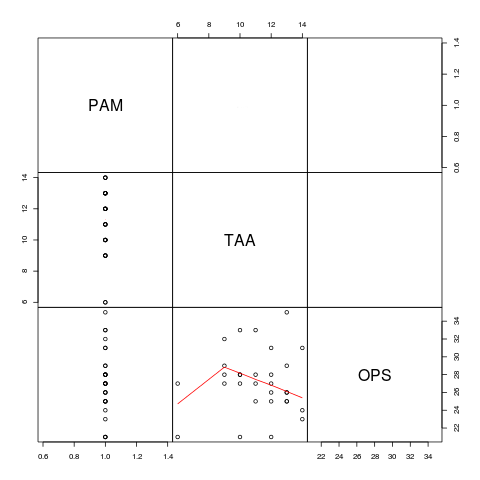
\includegraphics[scale=0.43]{include/appendix/fig/AppropriateDistributionofExpertise.png}}
{\caption{Appropriate Distribution of Expertise} 
\label{fig:ade_plot}}
\end{minipage}
\quad
\begin{minipage}[b]{0.43\linewidth}
\ffigbox[\FBwidth] {
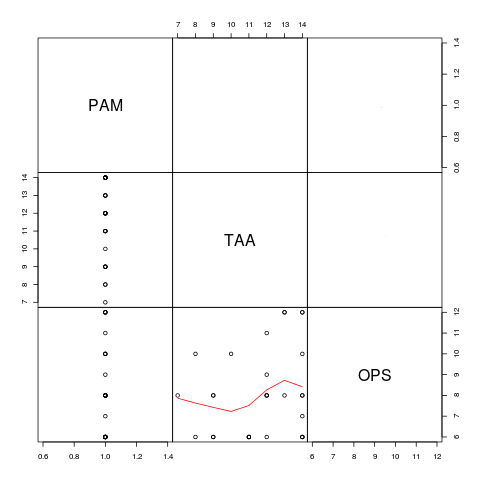
\includegraphics[scale=0.45]{include/appendix/fig/AdherencetoStandards.png}}
{\caption{Adherence to Standards} 
\label{fig:ads_plot}}
\end{minipage}

\begin{minipage}[b]{0.45\linewidth}
\ffigbox[\FBwidth] {
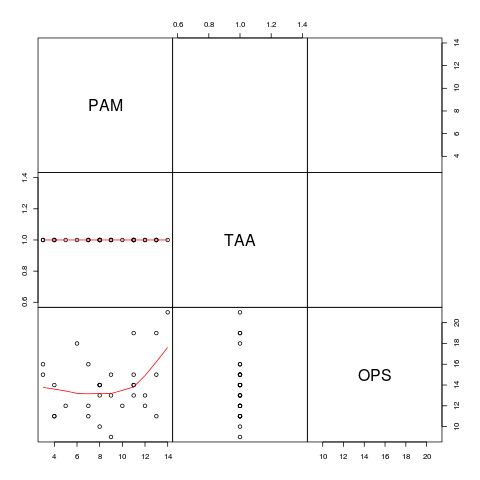
\includegraphics[scale=0.43]{include/appendix/fig/Client-DrivenIterations.png}}
{\caption{Client-Driven Iterations} 
\label{fig:cdi_plot}}
\end{minipage}
\quad
\begin{minipage}[b]{0.43\linewidth}
\ffigbox[\FBwidth] {
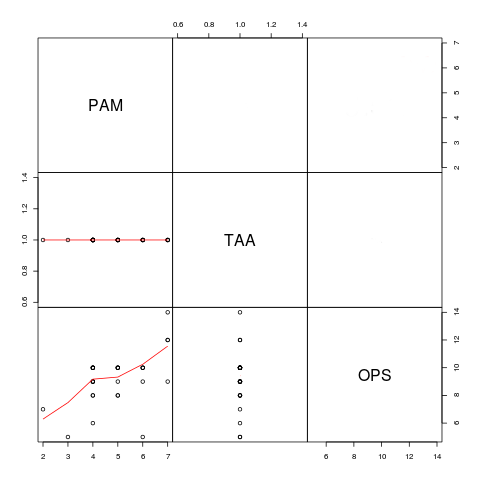
\includegraphics[scale=0.45]{include/appendix/fig/ContinuousFeedback.png}}
{\caption{Continuous Feedback} 
\label{fig:cf_plot}}
\end{minipage}

\begin{minipage}[b]{0.45\linewidth}
\ffigbox[\FBwidth] {
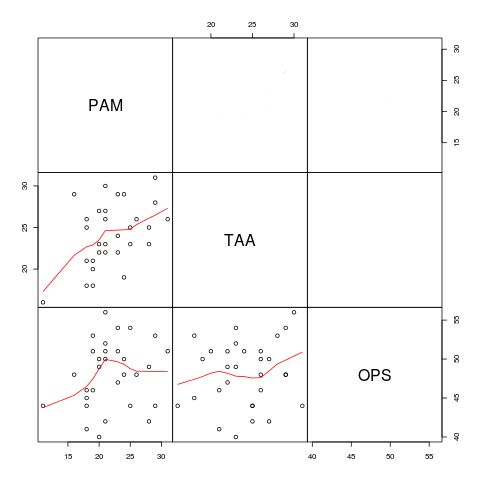
\includegraphics[scale=0.43]{include/appendix/fig/ContinuousIntegration.png}}
{\caption{Continuous Integration} 
\label{fig:ci_plot}}
\end{minipage}
\quad
\begin{minipage}[b]{0.43\linewidth}
\ffigbox[\FBwidth] {
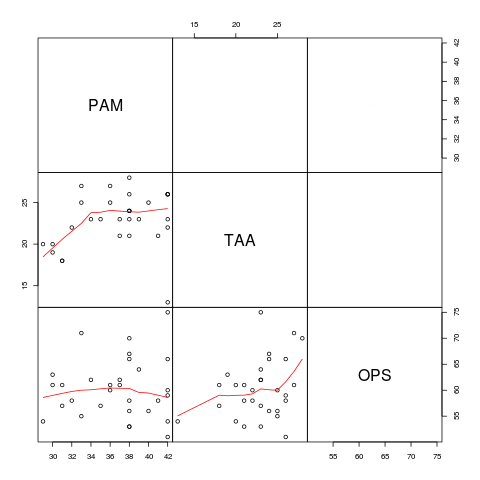
\includegraphics[scale=0.45]{include/appendix/fig/High-BandwidthCommunication.png}}
{\caption{High-Bandwidth Communication} 
\label{fig:hbc_plot}}
\end{minipage}

\begin{minipage}[b]{0.45\linewidth}
\ffigbox[\FBwidth] {
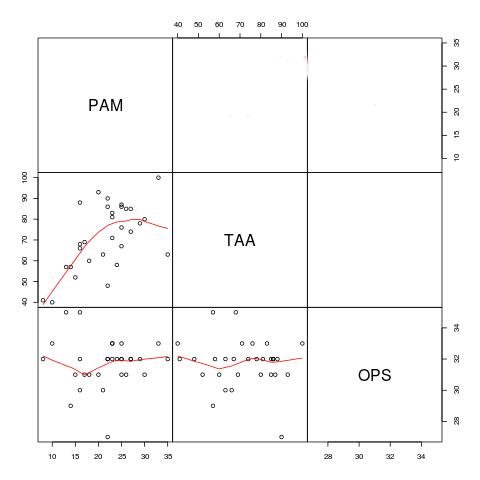
\includegraphics[scale=0.43]{include/appendix/fig/IterationProgressTrackingandReporting.png}}
{\caption{Iteration Progress Tracking and Reporting} 
\label{fig:iptr_plot}}
\end{minipage}
\quad
\begin{minipage}[b]{0.43\linewidth}
\ffigbox[\FBwidth] {
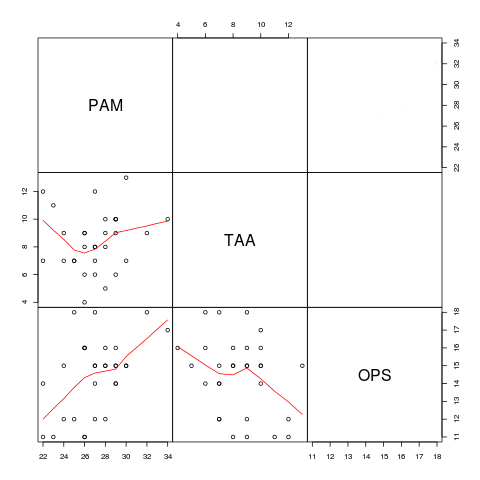
\includegraphics[scale=0.45]{include/appendix/fig/IterativeandIncrementalDevelopment.png}}
{\caption{Iterative and Incremental Development} 
\label{fig:iid_plot}}
\end{minipage}

\begin{minipage}[b]{0.45\linewidth}
\ffigbox[\FBwidth] {
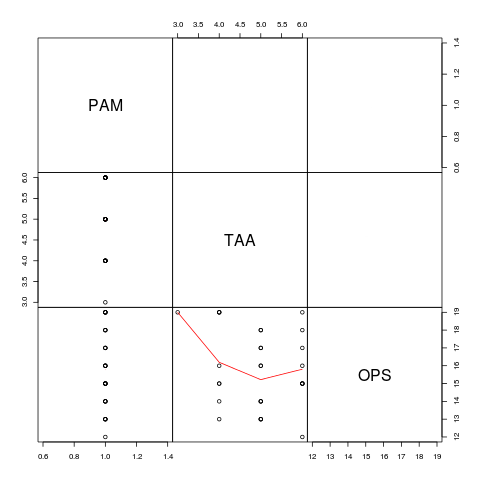
\includegraphics[scale=0.43]{include/appendix/fig/ProductBacklog.png}}
{\caption{Product Backlog} 
\label{fig:pb_plot}}
\end{minipage}
\quad
\begin{minipage}[b]{0.43\linewidth}
\ffigbox[\FBwidth] {
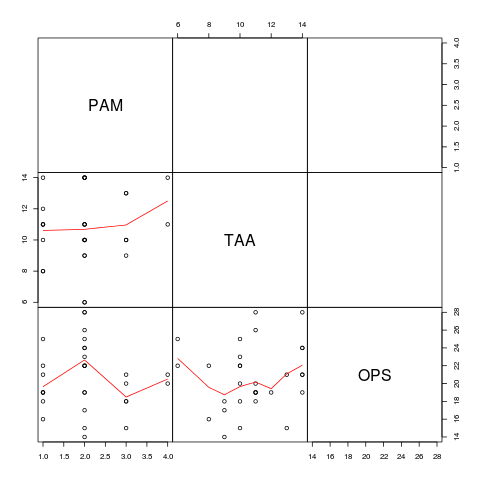
\includegraphics[scale=0.45]{include/appendix/fig/Refactoring.png}}
{\caption{Refactoring} 
\label{fig:ref_plot}}
\end{minipage}

\begin{minipage}[b]{0.45\linewidth}
\ffigbox[\FBwidth] {
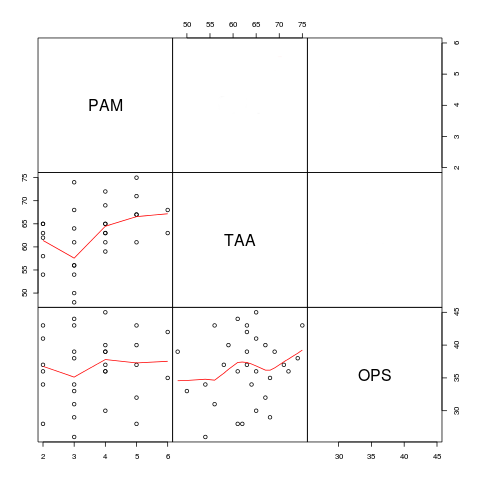
\includegraphics[scale=0.43]{include/appendix/fig/Self-OrganizingTeams.png}}
{\caption{Self-Organizing Teams} 
\label{fig:sot_plot}}
\end{minipage}
\quad
\begin{minipage}[b]{0.43\linewidth}
\ffigbox[\FBwidth] {
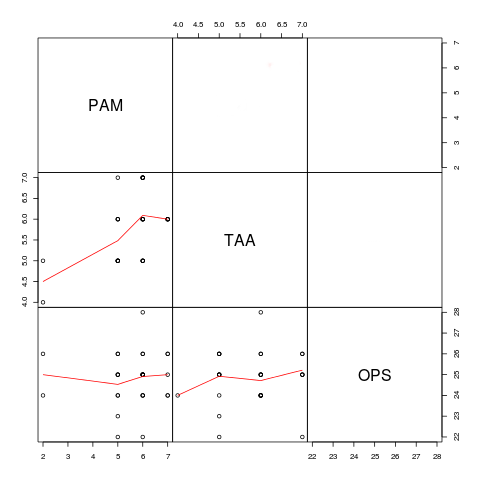
\includegraphics[scale=0.45]{include/appendix/fig/SmallerandFrequentProductReleases.png}}
{\caption{Smaller and Frequent Product Releases} 
\label{fig:sfpr_plot}}
\end{minipage}

\begin{minipage}[b]{0.45\linewidth}
\ffigbox[\FBwidth] {
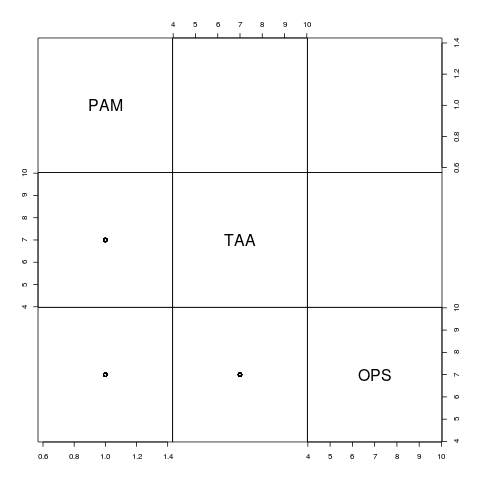
\includegraphics[scale=0.43]{include/appendix/fig/SoftwareConfigurationManagement.png}}
{\caption{Software Configuration Management} 
\label{fig:scm_plot}}
\end{minipage}
\quad
\begin{minipage}[b]{0.43\linewidth}
\ffigbox[\FBwidth] {
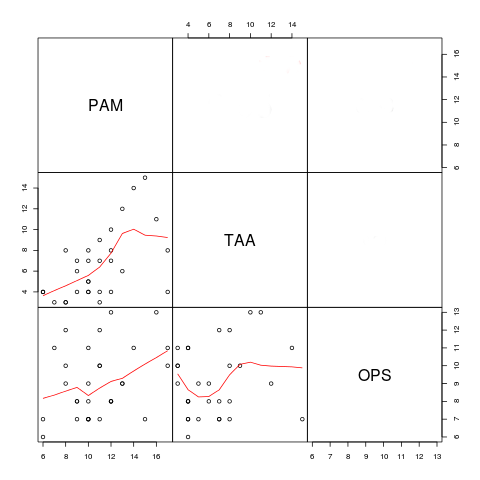
\includegraphics[scale=0.45]{include/appendix/fig/TestDrivenDevelopment.png}}
{\caption{Test Driven Development} 
\label{fig:tdd_plot}}
\end{minipage}




\end{appendices}
